\documentclass{beamer}

% Useful packages
\usepackage[utf8]{inputenc}
\usepackage{graphicx}
\usepackage{booktabs}
\usepackage{amsmath, amsfonts}
\usepackage{hyperref}

% Title metadata
\title[Short Title]{Hotwire Native}
\author{Aron Wolf}
\date{}

\titlegraphic{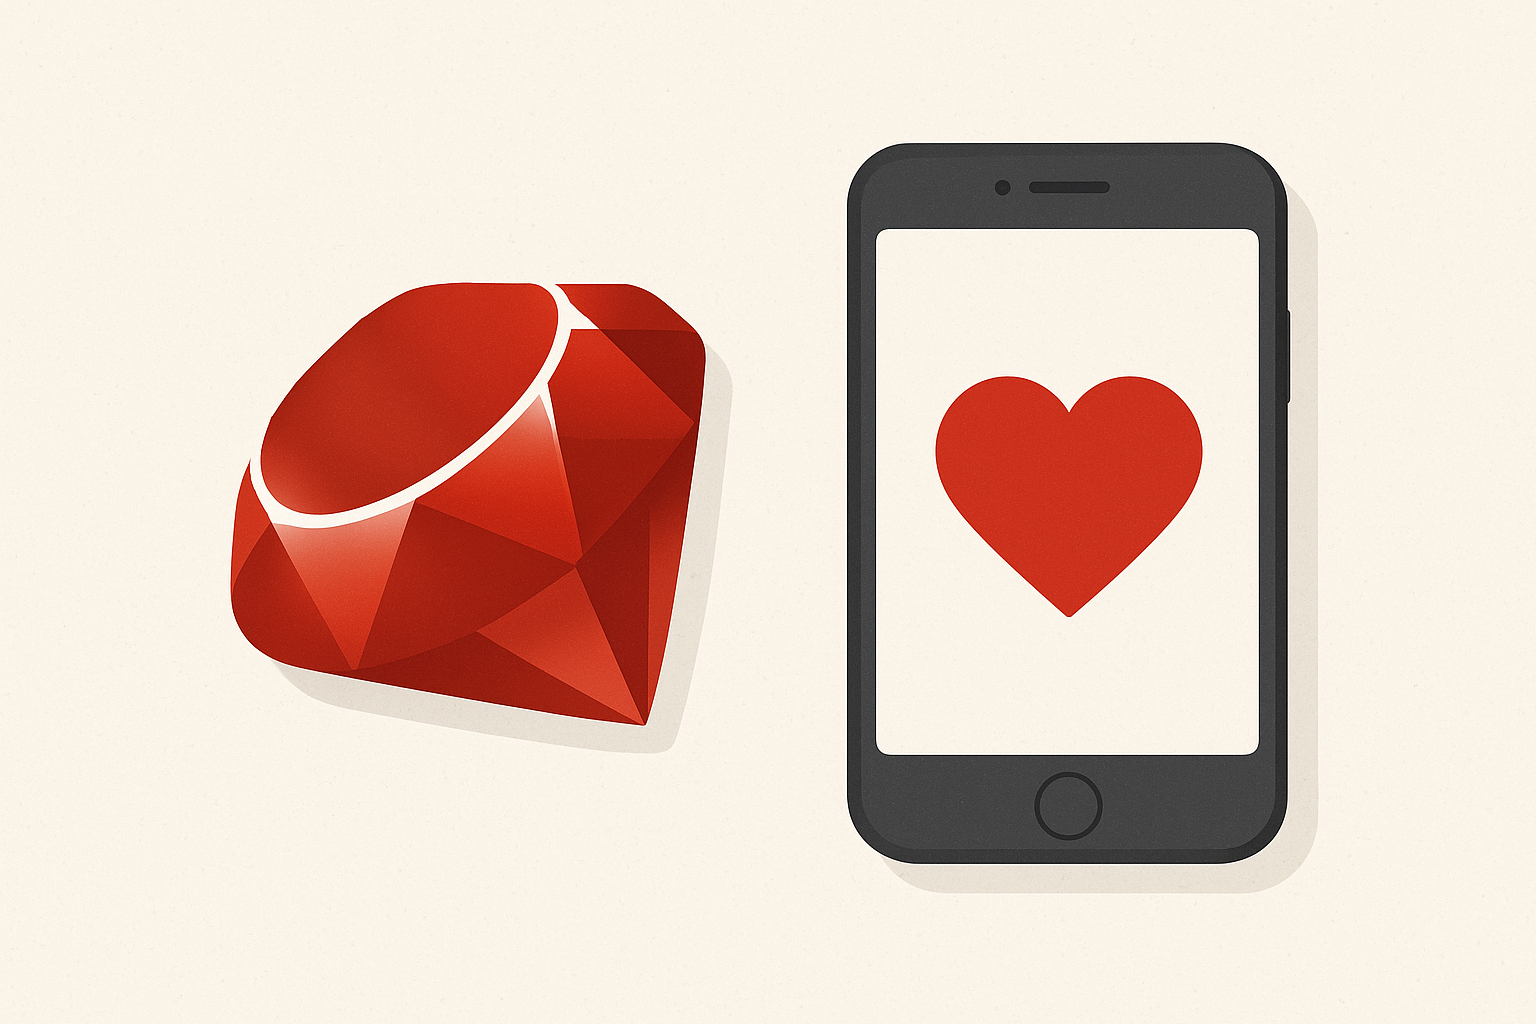
\includegraphics[height=.48\textheight]{images/ruby-love-mobile.png}}
\definecolor{background}{HTML}{fbf4e8}
\setbeamercolor{background canvas}{bg=background}
\setbeamertemplate{footline}[frame number]{}
\setbeamertemplate{navigation symbols}{}
\setbeamertemplate{footline}{}

\begin{document}

\begin{frame}
  \titlepage
\end{frame}

\section{Introduction}

\begin{frame}{Convert your fullstack Rails application into a mobile app}
  \begin{itemize}
    \item It was created by 37signals (the company that invented Ruby on Rails!).
    \item It allows you to convert your application into a mobile app.
  \end{itemize}
  \centering
  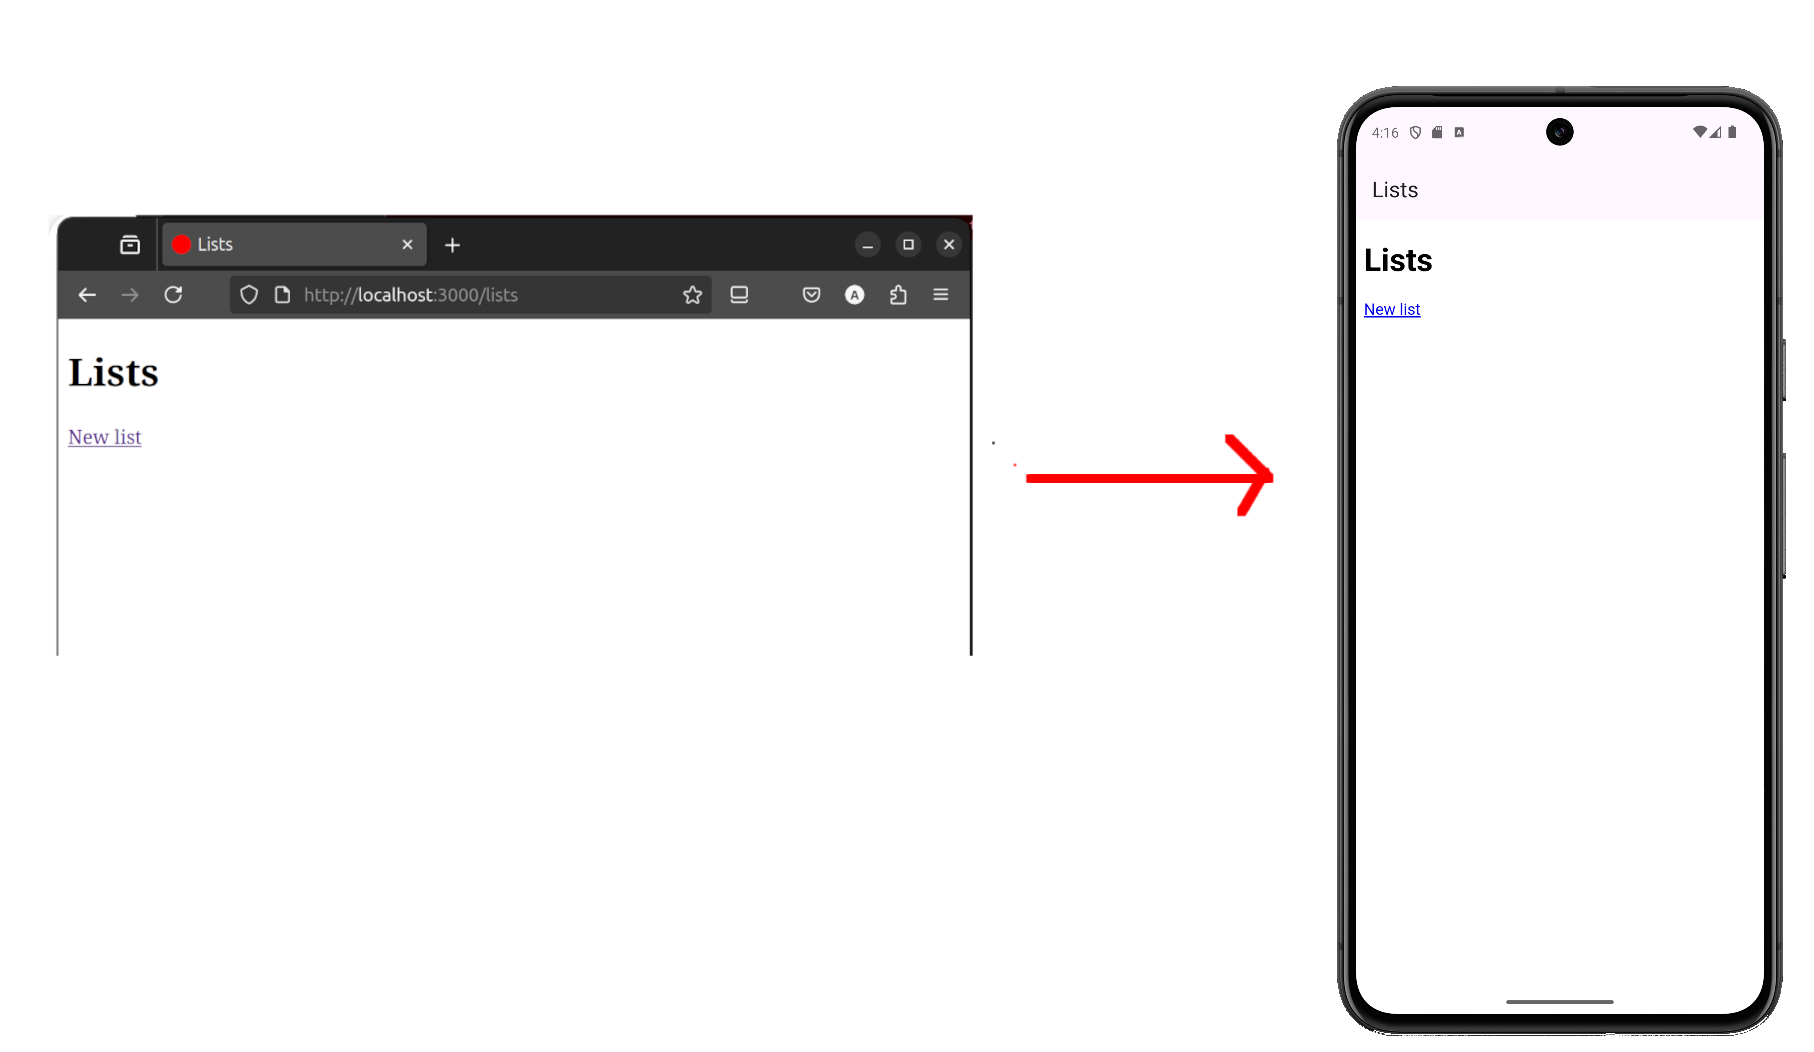
\includegraphics[width=0.8\linewidth]{images/convert-app.png}
\end{frame}

\begin{frame}{Why?}
  \begin{itemize}
    \item Maintaining multiple frontends is hard.
    \item This approach is more frequent than many think.
  \end{itemize}
\end{frame}

\section{Methodology}

\begin{frame}{Native feeling: mixes native elements and web views}

  \centering
  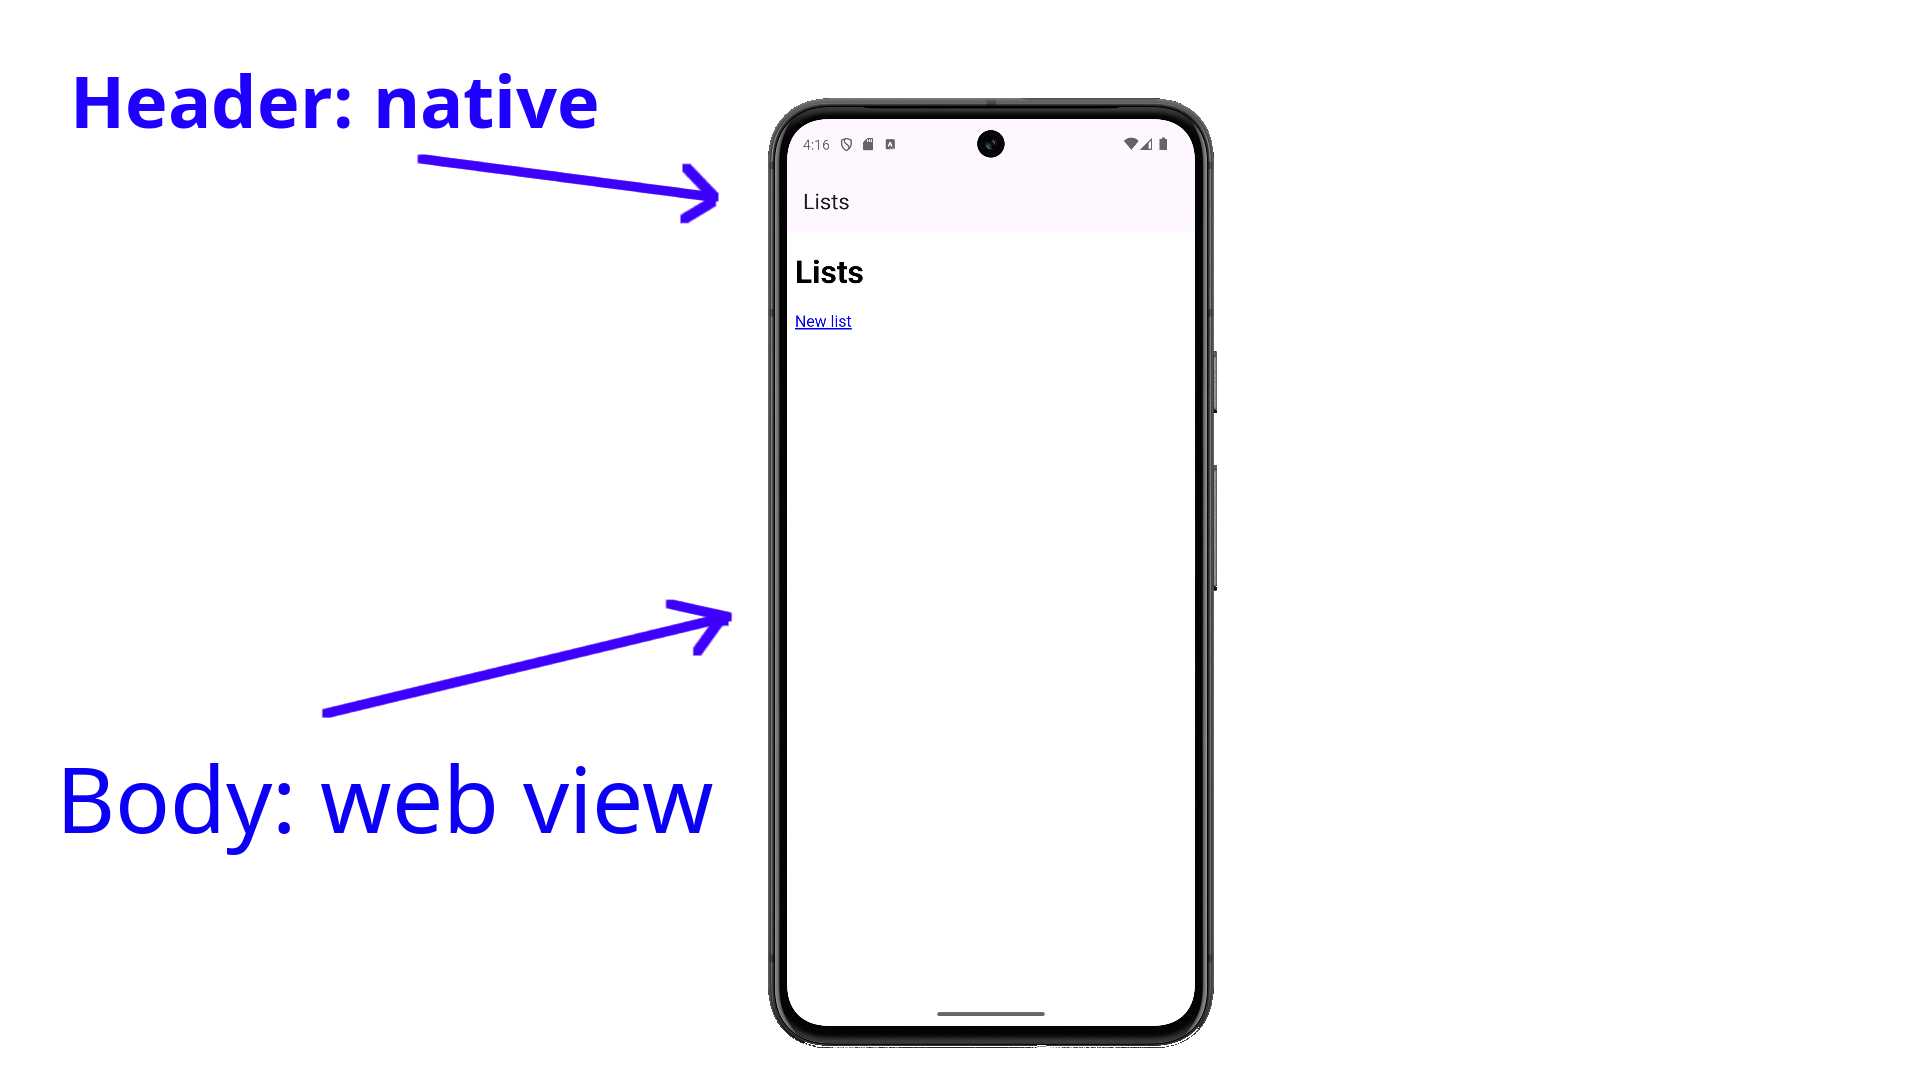
\includegraphics[width=0.8\linewidth]{images/header-body.png}
\end{frame}

\begin{frame}{Path Configuration}
  \centering
  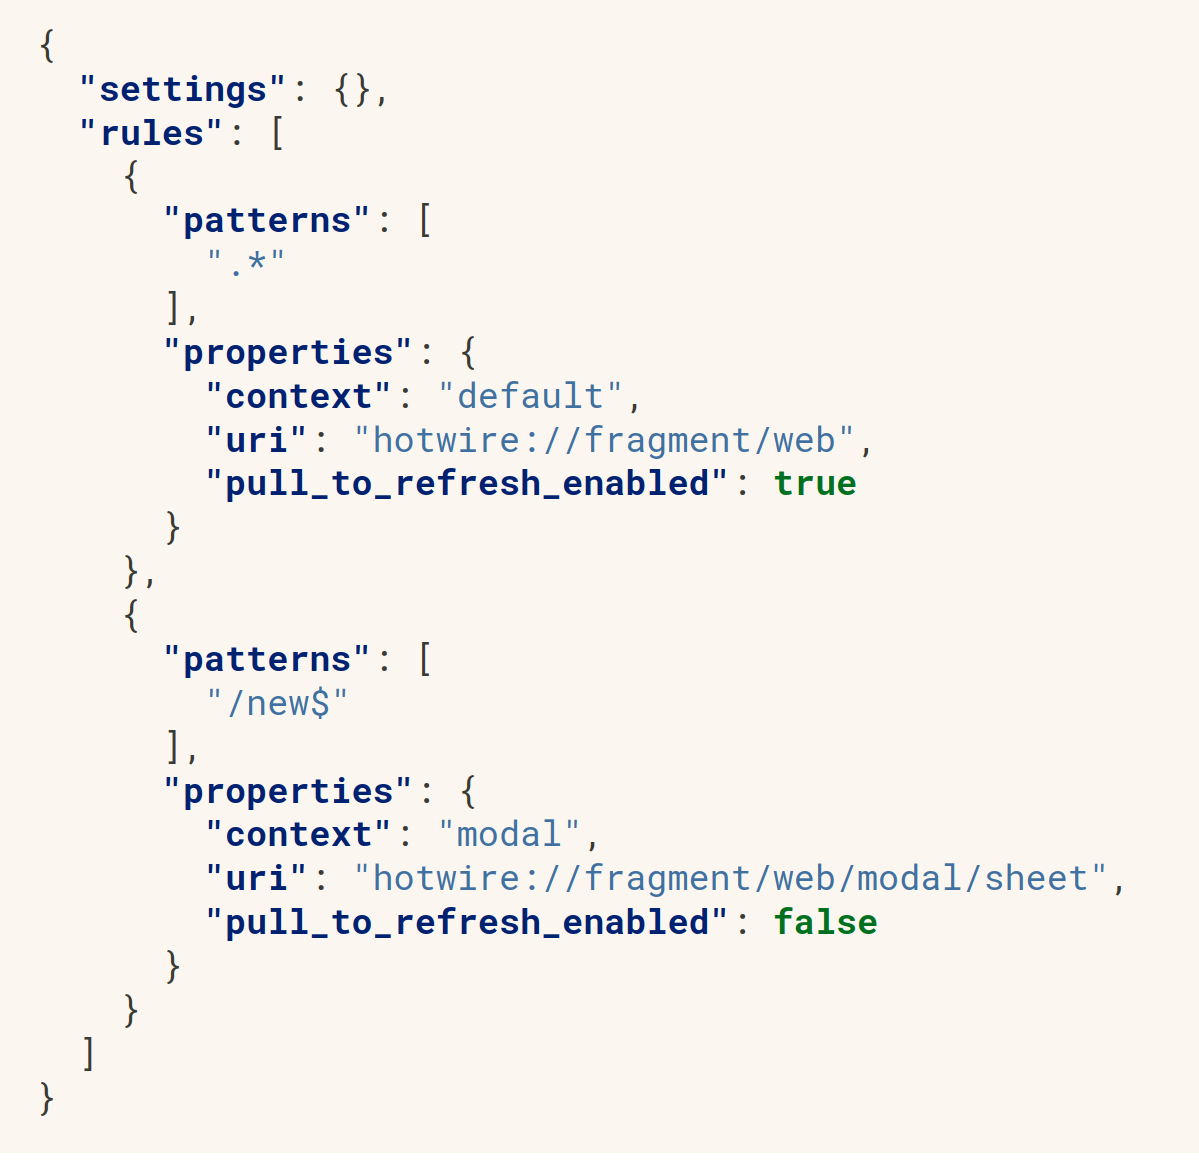
\includegraphics[width=0.8\linewidth]{images/path-configuration.png}
\end{frame}

\begin{frame}{Setup}
  https://native.hotwired.dev/android/getting-started
\end{frame}

\section{Results}

\begin{frame}{Debug}
  \centering
  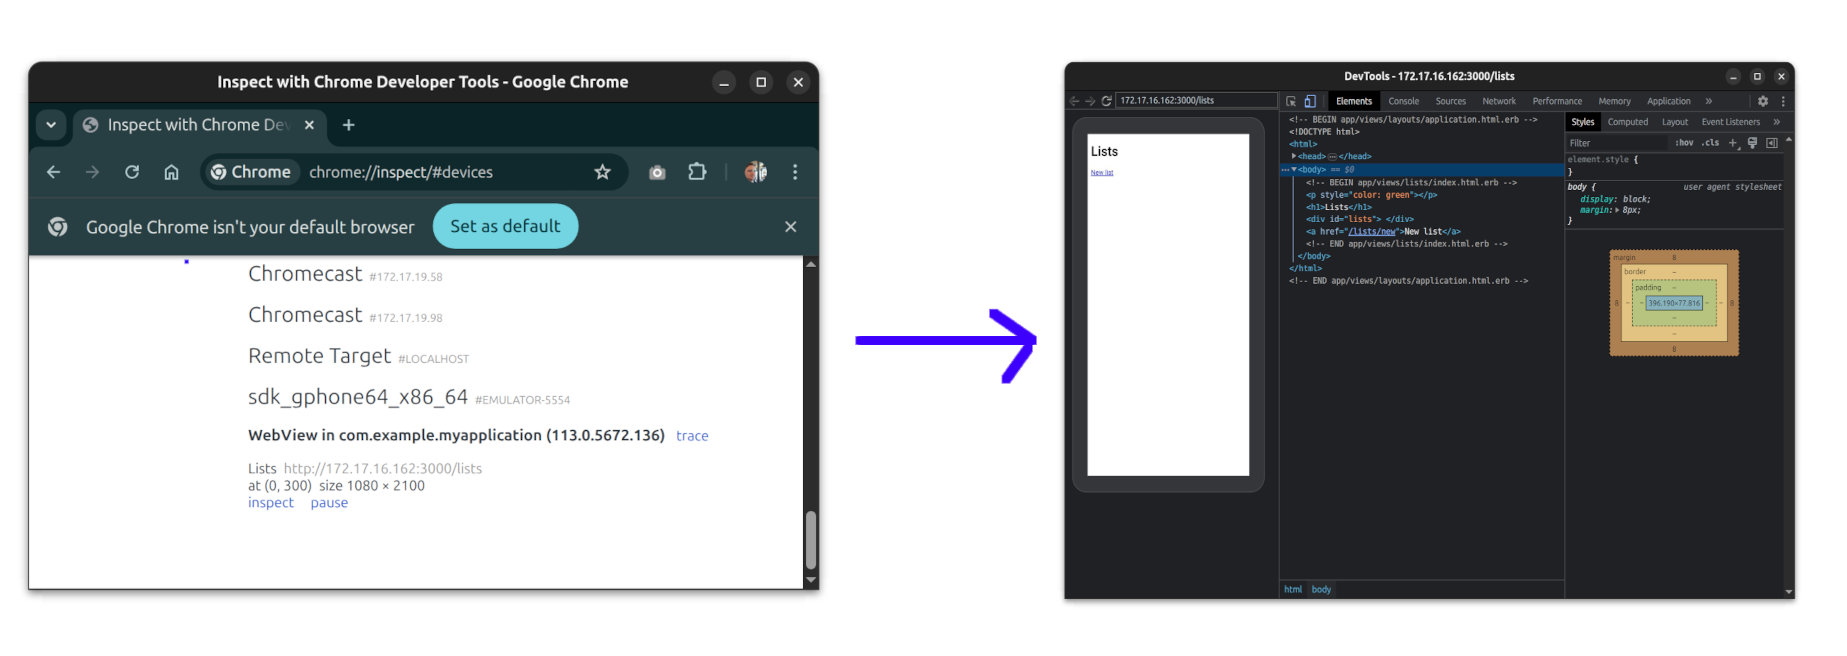
\includegraphics[width=1\linewidth]{images/debug.png}
\end{frame}


\begin{frame}{Thank You!}
  \centering
  \Large Questions? \\
  \vspace{1cm}
  \normalsize
  \href{your.email@example.com}{aronwolf90@gmail.com}
\end{frame}

\end{document}
